% Fragmento LaTeX: Arquitectura del sistema y flujo de ejecución
% Incluir en el TFM con: % Fragmento LaTeX: Arquitectura del sistema y flujo de ejecución
% Incluir en el TFM con: % Fragmento LaTeX: Arquitectura del sistema y flujo de ejecución
% Incluir en el TFM con: % Fragmento LaTeX: Arquitectura del sistema y flujo de ejecución
% Incluir en el TFM con: \input{docs/arquitectura_sistema}
% Rutas de figuras relativas al directorio raíz del TFM (ajustar \graphicspath si procede).
% Alternativa vectorial: uml_dominio_sin_titulo.pdf, uml_motor.pdf (exportar con PlantUML).

\subsection{Arquitectura del sistema propuesto y flujo de ejecución}
\label{subsec:arquitectura-sistema}

Para evitar el acoplamiento rígido de componentes---un defecto habitual en motores de simulación académicos---, el sistema se ha diseñado bajo un enfoque modular y orientado a objetos, distribuyendo las responsabilidades en bibliotecas independientes (\texttt{Asset}, \texttt{Portfolio}, \texttt{Random}, \texttt{InterestRate}, \texttt{MontecarloEngine} y \texttt{Metrics}). El flujo de vida del dato dentro del motor puede estructurarse en tres fases secuenciales: \emph{configuración}, \emph{orquestación y simulación}, y \emph{análisis de riesgo sobre la distribución empírica de P\&L} (cuantiles y métricas de cola).

A continuación se detallan las responsabilidades de los módulos principales. La Figura~\ref{fig:uml-dominio} recoge el \emph{modelo de dominio}; la Figura~\ref{fig:uml-motor}, el \emph{motor de simulación} y las métricas asociadas.

\begin{itemize}
  \item \textbf{Cápsula de configuración (\texttt{SimConfig}).}
  Estructura de datos ligera que centraliza los parámetros de la simulación y elimina variables codificadas en el código (\emph{hardcoded}).
  Almacena el horizonte temporal (\texttt{totalTime}), el número de pasos (\texttt{numSteps}), el tamaño muestral (\texttt{totalSims}), la matriz de correlación (\texttt{corrMatrix}), el paralelismo (\texttt{numCores}), el generador aleatorio (\texttt{rngType}, \texttt{rngSeed}), el \emph{layout} de la matriz de shocks (\texttt{matrixLayout}) y, de forma opcional, un modelo de tipos de interés (\texttt{rateModel}) y la estimación de errores estándar de VaR/ES (\texttt{computeStandardErrors}, \texttt{bootstrapReplications}, \texttt{sobolBatchCount}).
  Todos estos campos residen en memoria; \texttt{SimConfig} no gestiona rutas de ficheros de mercado.

  \item \textbf{Modelización de activos (\texttt{Asset} y derivadas).}
  La clase base abstracta \texttt{Asset} define la interfaz polimórfica de cualquier factor de riesgo.
  Las implementaciones concretas incluyen \texttt{GBMAsset} (movimiento browniano geométrico), \texttt{EuropeanOption}, \texttt{BarrierOption} (up-and-out call) y \texttt{CouponBond} (modo YTM o precio vía modelo de tipos).
  El método \texttt{simulateFinalValue} constituye el \emph{hot path} invocado por la cartera;  \texttt{generatePath} se reserva para tests y análisis (\emph{cold path}).
  Esta jerarquía permite que el motor sea agnóstico respecto al modelo estocástico de cada instrumento.

  \item \textbf{Agregación en cartera (\texttt{Portfolio}, \texttt{Position}).}
  \texttt{Portfolio} agrupa posiciones (\texttt{Position}), cada una con un \texttt{shared\_ptr<Asset>} y una cantidad.
  El método \texttt{simulatePathPnL} calcula el P\&L de una trayectoria: valora cada activo mediante \texttt{simulateFinalValue}, aplica descuento opcional con \texttt{InterestRateModel} y resta el valor inicial de la cartera.

  \item \textbf{Tipos de interés (\texttt{InterestRateModel}, \texttt{HullWhiteModel}).}
  Interfaz abstracta para simular la trayectoria del tipo corto, descontar flujos y valorar bonos.
  La implementación \texttt{HullWhiteModel} compone una \texttt{YieldCurve} de mercado.
  Su uso es opcional: cuando \texttt{SimConfig.rateModel} está activo, la matriz de correlación incorpora un factor adicional para el driver browniano del tipo.

  \item \textbf{Aleatoriedad (\texttt{RandomGenerator} y utilidades).}
  \texttt{MersenneTwisterGen} y \texttt{BoostSobolGenerator} implementan la interfaz \texttt{RandomGenerator}.
  El motor selecciona el generador según \texttt{rngType}: Mersenne Twister, variables antitéticas (pares $(Z,-Z)$) o secuencias de Sobol.
  En el modo Sobol, \texttt{BoostSobolGenerator} transforma uniformes cuasi-aleatorios mediante \texttt{MathUtils::inverseNormalCDF} y \texttt{MonteCarloEngine} aplica \texttt{BrownianBridge} por factor antes de la correlación.

  \item \textbf{Núcleo de orquestación (\texttt{MonteCarloEngine}).}
  Punto de entrada \texttt{run(const Portfolio\&, const SimConfig\&)}.
  Recibe una cartera ya construida (no la instancia), descompone la correlación con Cholesky ($Z_{\mathrm{corr}} = L Z_{\mathrm{indep}}$), paraleliza batches con \texttt{std::async} y coordina RNG, trayectorias de tipos y llamadas a \texttt{Portfolio::simulatePathPnL}.
  Es aquí donde se integran las técnicas de reducción de varianza y el bucle crítico de Monte Carlo.

  \item \textbf{Consumidor de riesgo (\texttt{RiskCalculator}, \texttt{MonteCarloErrorPolicy}).}
  Módulo de análisis \emph{posterior} a la simulación.
  Recibe el \emph{vector} de P\&L simulados (no una matriz), los ordena y calcula VaR$_\alpha$ y ES$_\alpha$ empíricos para $\alpha \in (0,1)$.
  Cuando \texttt{computeStandardErrors} está activo, \texttt{MonteCarloErrorPolicy} estima errores estándar según el esquema asociado al \texttt{rngType} (muestras independientes, pares antitéticos o medias por lotes Sobol), devolviendo \texttt{RiskEstimate} con valor y error.
  Las operaciones estadísticas quedan así aisladas de la lógica de simulación.
\end{itemize}

Como se aprecia en las Figuras~\ref{fig:uml-dominio} y~\ref{fig:uml-motor}, la interacción entre componentes modela el flujo de dependencias del software: el dominio financiero (activos, cartera y tipos) se desacopla del motor, que a su vez delega las métricas en \texttt{Metrics}.
El orquestador central gobierna el ciclo de vida de la simulación sin violar el principio de responsabilidad única.

\begin{figure}[htbp]
  \centering
  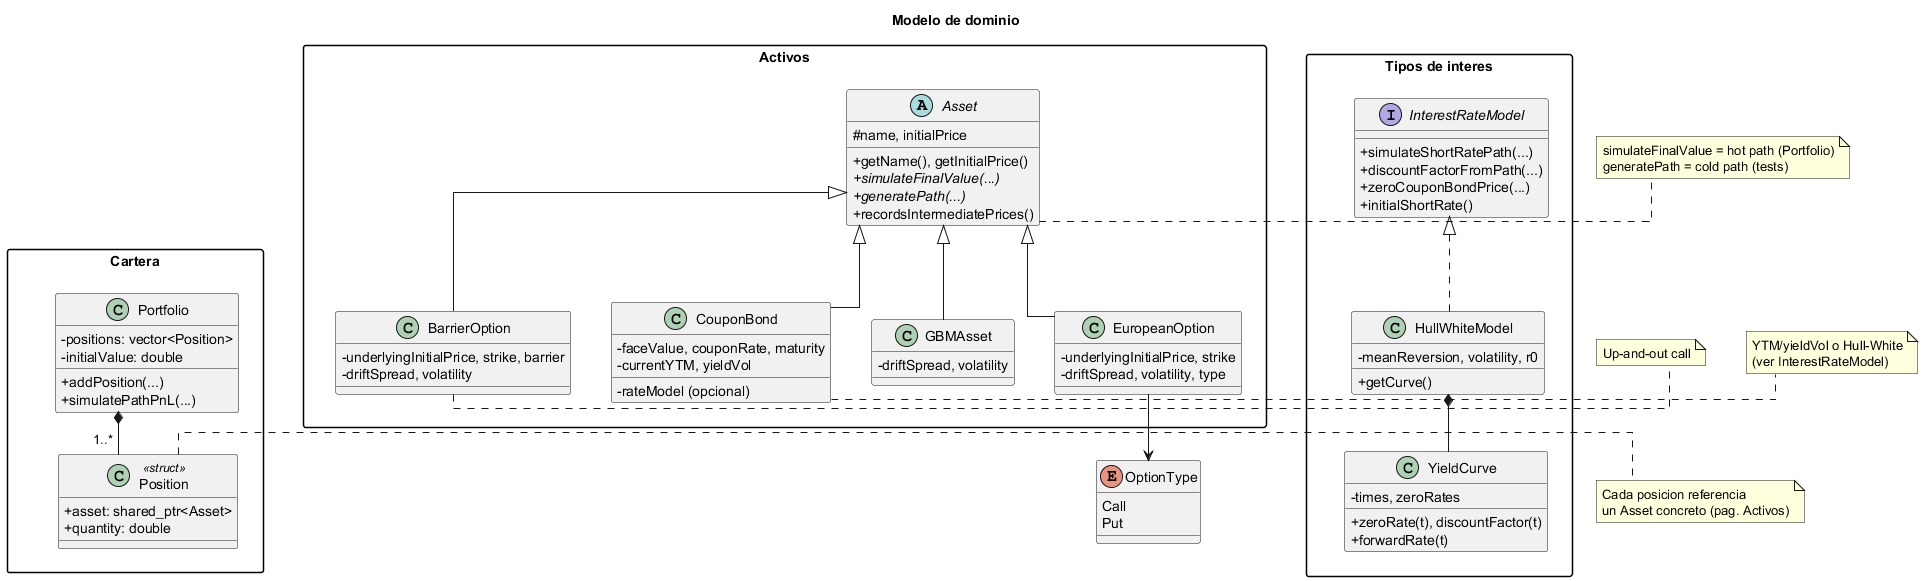
\includegraphics[width=\textwidth]{graphics/uml/uml_dominio.png}
  \caption{Modelo de dominio del motor: jerarquía de activos, agregación en cartera (\texttt{Portfolio}--\texttt{Position}) y modelado de tipos de interés.}
  \label{fig:uml-dominio}
\end{figure}

\begin{figure}[htbp]
  \centering
  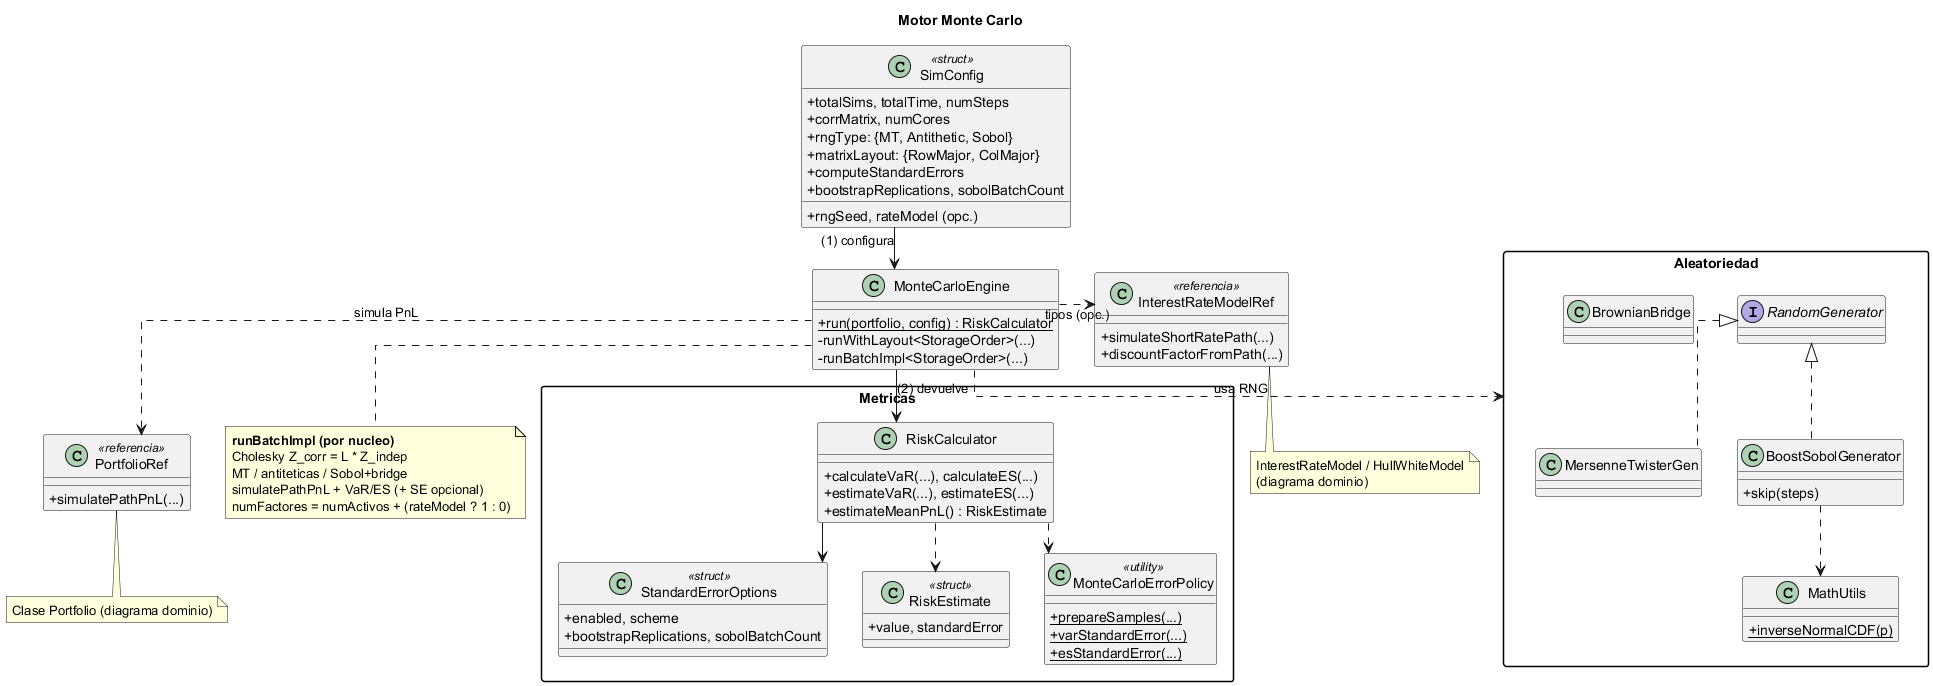
\includegraphics[width=\textwidth]{graphics/uml/uml_motor.png}
  \caption{Motor Monte Carlo: configuración (\texttt{SimConfig}), orquestación (\texttt{MonteCarloEngine}), generación aleatoria y cálculo de métricas de riesgo.}
  \label{fig:uml-motor}
\end{figure}

Este desacoplamiento arquitectónico garantiza flexibilidad funcional.
Modificar el horizonte temporal (p.\,ej.\ 1 día, 10 días o 1 año), el número de simulaciones, el generador aleatorio, la matriz de correlación o el modelo de tipos se reduce a reconfigurar \texttt{SimConfig} en los entornos de prueba (\texttt{test\_acciones.cpp} y \texttt{test\_montecarloEngine.cpp}), sin alterar la lógica interna del motor ni recompilar binarios de producción más allá de la reejecución de los tests de integración.

% Rutas de figuras relativas al directorio raíz del TFM (ajustar \graphicspath si procede).
% Alternativa vectorial: uml_dominio_sin_titulo.pdf, uml_motor.pdf (exportar con PlantUML).

\subsection{Arquitectura del sistema propuesto y flujo de ejecución}
\label{subsec:arquitectura-sistema}

Para evitar el acoplamiento rígido de componentes---un defecto habitual en motores de simulación académicos---, el sistema se ha diseñado bajo un enfoque modular y orientado a objetos, distribuyendo las responsabilidades en bibliotecas independientes (\texttt{Asset}, \texttt{Portfolio}, \texttt{Random}, \texttt{InterestRate}, \texttt{MontecarloEngine} y \texttt{Metrics}). El flujo de vida del dato dentro del motor puede estructurarse en tres fases secuenciales: \emph{configuración}, \emph{orquestación y simulación}, y \emph{análisis de riesgo sobre la distribución empírica de P\&L} (cuantiles y métricas de cola).

A continuación se detallan las responsabilidades de los módulos principales. La Figura~\ref{fig:uml-dominio} recoge el \emph{modelo de dominio}; la Figura~\ref{fig:uml-motor}, el \emph{motor de simulación} y las métricas asociadas.

\begin{itemize}
  \item \textbf{Cápsula de configuración (\texttt{SimConfig}).}
  Estructura de datos ligera que centraliza los parámetros de la simulación y elimina variables codificadas en el código (\emph{hardcoded}).
  Almacena el horizonte temporal (\texttt{totalTime}), el número de pasos (\texttt{numSteps}), el tamaño muestral (\texttt{totalSims}), la matriz de correlación (\texttt{corrMatrix}), el paralelismo (\texttt{numCores}), el generador aleatorio (\texttt{rngType}, \texttt{rngSeed}), el \emph{layout} de la matriz de shocks (\texttt{matrixLayout}) y, de forma opcional, un modelo de tipos de interés (\texttt{rateModel}) y la estimación de errores estándar de VaR/ES (\texttt{computeStandardErrors}, \texttt{bootstrapReplications}, \texttt{sobolBatchCount}).
  Todos estos campos residen en memoria; \texttt{SimConfig} no gestiona rutas de ficheros de mercado.

  \item \textbf{Modelización de activos (\texttt{Asset} y derivadas).}
  La clase base abstracta \texttt{Asset} define la interfaz polimórfica de cualquier factor de riesgo.
  Las implementaciones concretas incluyen \texttt{GBMAsset} (movimiento browniano geométrico), \texttt{EuropeanOption}, \texttt{BarrierOption} (up-and-out call) y \texttt{CouponBond} (modo YTM o precio vía modelo de tipos).
  El método \texttt{simulateFinalValue} constituye el \emph{hot path} invocado por la cartera;  \texttt{generatePath} se reserva para tests y análisis (\emph{cold path}).
  Esta jerarquía permite que el motor sea agnóstico respecto al modelo estocástico de cada instrumento.

  \item \textbf{Agregación en cartera (\texttt{Portfolio}, \texttt{Position}).}
  \texttt{Portfolio} agrupa posiciones (\texttt{Position}), cada una con un \texttt{shared\_ptr<Asset>} y una cantidad.
  El método \texttt{simulatePathPnL} calcula el P\&L de una trayectoria: valora cada activo mediante \texttt{simulateFinalValue}, aplica descuento opcional con \texttt{InterestRateModel} y resta el valor inicial de la cartera.

  \item \textbf{Tipos de interés (\texttt{InterestRateModel}, \texttt{HullWhiteModel}).}
  Interfaz abstracta para simular la trayectoria del tipo corto, descontar flujos y valorar bonos.
  La implementación \texttt{HullWhiteModel} compone una \texttt{YieldCurve} de mercado.
  Su uso es opcional: cuando \texttt{SimConfig.rateModel} está activo, la matriz de correlación incorpora un factor adicional para el driver browniano del tipo.

  \item \textbf{Aleatoriedad (\texttt{RandomGenerator} y utilidades).}
  \texttt{MersenneTwisterGen} y \texttt{BoostSobolGenerator} implementan la interfaz \texttt{RandomGenerator}.
  El motor selecciona el generador según \texttt{rngType}: Mersenne Twister, variables antitéticas (pares $(Z,-Z)$) o secuencias de Sobol.
  En el modo Sobol, \texttt{BoostSobolGenerator} transforma uniformes cuasi-aleatorios mediante \texttt{MathUtils::inverseNormalCDF} y \texttt{MonteCarloEngine} aplica \texttt{BrownianBridge} por factor antes de la correlación.

  \item \textbf{Núcleo de orquestación (\texttt{MonteCarloEngine}).}
  Punto de entrada \texttt{run(const Portfolio\&, const SimConfig\&)}.
  Recibe una cartera ya construida (no la instancia), descompone la correlación con Cholesky ($Z_{\mathrm{corr}} = L Z_{\mathrm{indep}}$), paraleliza batches con \texttt{std::async} y coordina RNG, trayectorias de tipos y llamadas a \texttt{Portfolio::simulatePathPnL}.
  Es aquí donde se integran las técnicas de reducción de varianza y el bucle crítico de Monte Carlo.

  \item \textbf{Consumidor de riesgo (\texttt{RiskCalculator}, \texttt{MonteCarloErrorPolicy}).}
  Módulo de análisis \emph{posterior} a la simulación.
  Recibe el \emph{vector} de P\&L simulados (no una matriz), los ordena y calcula VaR$_\alpha$ y ES$_\alpha$ empíricos para $\alpha \in (0,1)$.
  Cuando \texttt{computeStandardErrors} está activo, \texttt{MonteCarloErrorPolicy} estima errores estándar según el esquema asociado al \texttt{rngType} (muestras independientes, pares antitéticos o medias por lotes Sobol), devolviendo \texttt{RiskEstimate} con valor y error.
  Las operaciones estadísticas quedan así aisladas de la lógica de simulación.
\end{itemize}

Como se aprecia en las Figuras~\ref{fig:uml-dominio} y~\ref{fig:uml-motor}, la interacción entre componentes modela el flujo de dependencias del software: el dominio financiero (activos, cartera y tipos) se desacopla del motor, que a su vez delega las métricas en \texttt{Metrics}.
El orquestador central gobierna el ciclo de vida de la simulación sin violar el principio de responsabilidad única.

\begin{figure}[htbp]
  \centering
  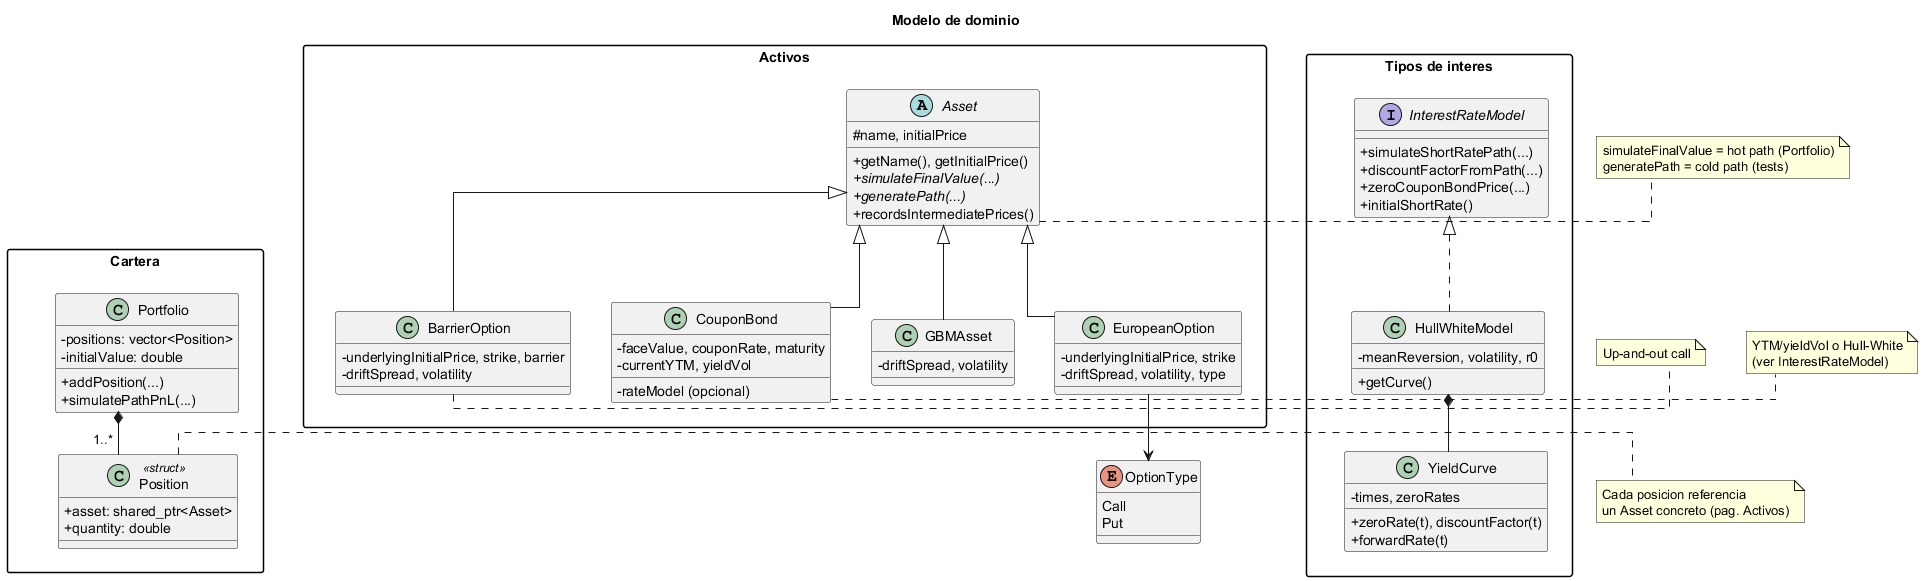
\includegraphics[width=\textwidth]{graphics/uml/uml_dominio.png}
  \caption{Modelo de dominio del motor: jerarquía de activos, agregación en cartera (\texttt{Portfolio}--\texttt{Position}) y modelado de tipos de interés.}
  \label{fig:uml-dominio}
\end{figure}

\begin{figure}[htbp]
  \centering
  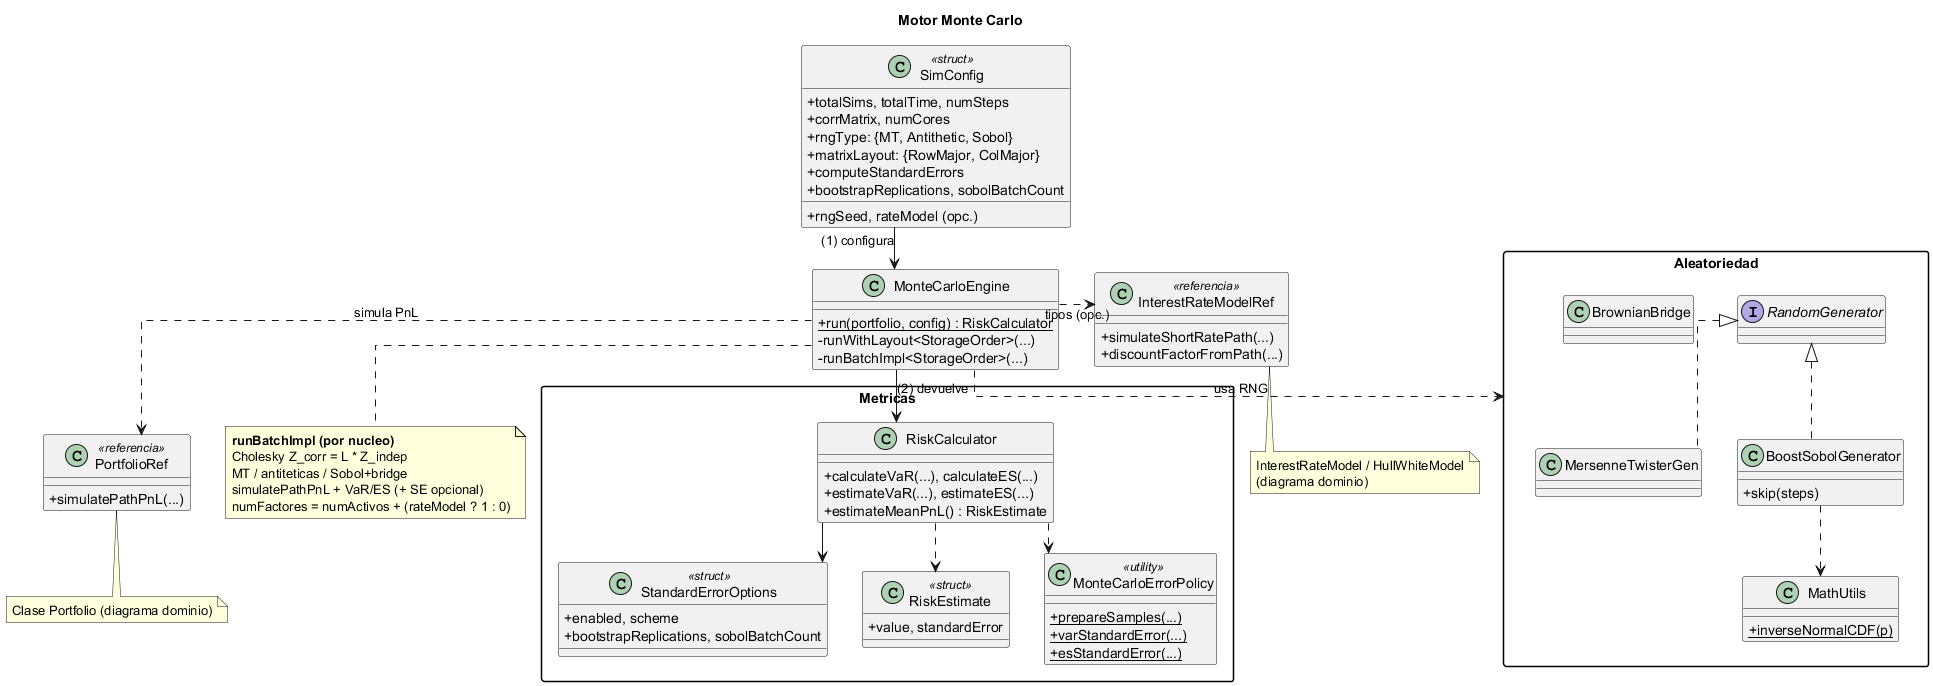
\includegraphics[width=\textwidth]{graphics/uml/uml_motor.png}
  \caption{Motor Monte Carlo: configuración (\texttt{SimConfig}), orquestación (\texttt{MonteCarloEngine}), generación aleatoria y cálculo de métricas de riesgo.}
  \label{fig:uml-motor}
\end{figure}

Este desacoplamiento arquitectónico garantiza flexibilidad funcional.
Modificar el horizonte temporal (p.\,ej.\ 1 día, 10 días o 1 año), el número de simulaciones, el generador aleatorio, la matriz de correlación o el modelo de tipos se reduce a reconfigurar \texttt{SimConfig} en los entornos de prueba (\texttt{test\_acciones.cpp} y \texttt{test\_montecarloEngine.cpp}), sin alterar la lógica interna del motor ni recompilar binarios de producción más allá de la reejecución de los tests de integración.

% Rutas de figuras relativas al directorio raíz del TFM (ajustar \graphicspath si procede).
% Alternativa vectorial: uml_dominio_sin_titulo.pdf, uml_motor.pdf (exportar con PlantUML).

\subsection{Arquitectura del sistema propuesto y flujo de ejecución}
\label{subsec:arquitectura-sistema}

Para evitar el acoplamiento rígido de componentes---un defecto habitual en motores de simulación académicos---, el sistema se ha diseñado bajo un enfoque modular y orientado a objetos, distribuyendo las responsabilidades en bibliotecas independientes (\texttt{Asset}, \texttt{Portfolio}, \texttt{Random}, \texttt{InterestRate}, \texttt{MontecarloEngine} y \texttt{Metrics}). El flujo de vida del dato dentro del motor puede estructurarse en tres fases secuenciales: \emph{configuración}, \emph{orquestación y simulación}, y \emph{análisis de riesgo sobre la distribución empírica de P\&L} (cuantiles y métricas de cola).

A continuación se detallan las responsabilidades de los módulos principales. La Figura~\ref{fig:uml-dominio} recoge el \emph{modelo de dominio}; la Figura~\ref{fig:uml-motor}, el \emph{motor de simulación} y las métricas asociadas.

\begin{itemize}
  \item \textbf{Cápsula de configuración (\texttt{SimConfig}).}
  Estructura de datos ligera que centraliza los parámetros de la simulación y elimina variables codificadas en el código (\emph{hardcoded}).
  Almacena el horizonte temporal (\texttt{totalTime}), el número de pasos (\texttt{numSteps}), el tamaño muestral (\texttt{totalSims}), la matriz de correlación (\texttt{corrMatrix}), el paralelismo (\texttt{numCores}), el generador aleatorio (\texttt{rngType}, \texttt{rngSeed}), el \emph{layout} de la matriz de shocks (\texttt{matrixLayout}) y, de forma opcional, un modelo de tipos de interés (\texttt{rateModel}) y la estimación de errores estándar de VaR/ES (\texttt{computeStandardErrors}, \texttt{bootstrapReplications}, \texttt{sobolBatchCount}).
  Todos estos campos residen en memoria; \texttt{SimConfig} no gestiona rutas de ficheros de mercado.

  \item \textbf{Modelización de activos (\texttt{Asset} y derivadas).}
  La clase base abstracta \texttt{Asset} define la interfaz polimórfica de cualquier factor de riesgo.
  Las implementaciones concretas incluyen \texttt{GBMAsset} (movimiento browniano geométrico), \texttt{EuropeanOption}, \texttt{BarrierOption} (up-and-out call) y \texttt{CouponBond} (modo YTM o precio vía modelo de tipos).
  El método \texttt{simulateFinalValue} constituye el \emph{hot path} invocado por la cartera;  \texttt{generatePath} se reserva para tests y análisis (\emph{cold path}).
  Esta jerarquía permite que el motor sea agnóstico respecto al modelo estocástico de cada instrumento.

  \item \textbf{Agregación en cartera (\texttt{Portfolio}, \texttt{Position}).}
  \texttt{Portfolio} agrupa posiciones (\texttt{Position}), cada una con un \texttt{shared\_ptr<Asset>} y una cantidad.
  El método \texttt{simulatePathPnL} calcula el P\&L de una trayectoria: valora cada activo mediante \texttt{simulateFinalValue}, aplica descuento opcional con \texttt{InterestRateModel} y resta el valor inicial de la cartera.

  \item \textbf{Tipos de interés (\texttt{InterestRateModel}, \texttt{HullWhiteModel}).}
  Interfaz abstracta para simular la trayectoria del tipo corto, descontar flujos y valorar bonos.
  La implementación \texttt{HullWhiteModel} compone una \texttt{YieldCurve} de mercado.
  Su uso es opcional: cuando \texttt{SimConfig.rateModel} está activo, la matriz de correlación incorpora un factor adicional para el driver browniano del tipo.

  \item \textbf{Aleatoriedad (\texttt{RandomGenerator} y utilidades).}
  \texttt{MersenneTwisterGen} y \texttt{BoostSobolGenerator} implementan la interfaz \texttt{RandomGenerator}.
  El motor selecciona el generador según \texttt{rngType}: Mersenne Twister, variables antitéticas (pares $(Z,-Z)$) o secuencias de Sobol.
  En el modo Sobol, \texttt{BoostSobolGenerator} transforma uniformes cuasi-aleatorios mediante \texttt{MathUtils::inverseNormalCDF} y \texttt{MonteCarloEngine} aplica \texttt{BrownianBridge} por factor antes de la correlación.

  \item \textbf{Núcleo de orquestación (\texttt{MonteCarloEngine}).}
  Punto de entrada \texttt{run(const Portfolio\&, const SimConfig\&)}.
  Recibe una cartera ya construida (no la instancia), descompone la correlación con Cholesky ($Z_{\mathrm{corr}} = L Z_{\mathrm{indep}}$), paraleliza batches con \texttt{std::async} y coordina RNG, trayectorias de tipos y llamadas a \texttt{Portfolio::simulatePathPnL}.
  Es aquí donde se integran las técnicas de reducción de varianza y el bucle crítico de Monte Carlo.

  \item \textbf{Consumidor de riesgo (\texttt{RiskCalculator}, \texttt{MonteCarloErrorPolicy}).}
  Módulo de análisis \emph{posterior} a la simulación.
  Recibe el \emph{vector} de P\&L simulados (no una matriz), los ordena y calcula VaR$_\alpha$ y ES$_\alpha$ empíricos para $\alpha \in (0,1)$.
  Cuando \texttt{computeStandardErrors} está activo, \texttt{MonteCarloErrorPolicy} estima errores estándar según el esquema asociado al \texttt{rngType} (muestras independientes, pares antitéticos o medias por lotes Sobol), devolviendo \texttt{RiskEstimate} con valor y error.
  Las operaciones estadísticas quedan así aisladas de la lógica de simulación.
\end{itemize}

Como se aprecia en las Figuras~\ref{fig:uml-dominio} y~\ref{fig:uml-motor}, la interacción entre componentes modela el flujo de dependencias del software: el dominio financiero (activos, cartera y tipos) se desacopla del motor, que a su vez delega las métricas en \texttt{Metrics}.
El orquestador central gobierna el ciclo de vida de la simulación sin violar el principio de responsabilidad única.

\begin{figure}[htbp]
  \centering
  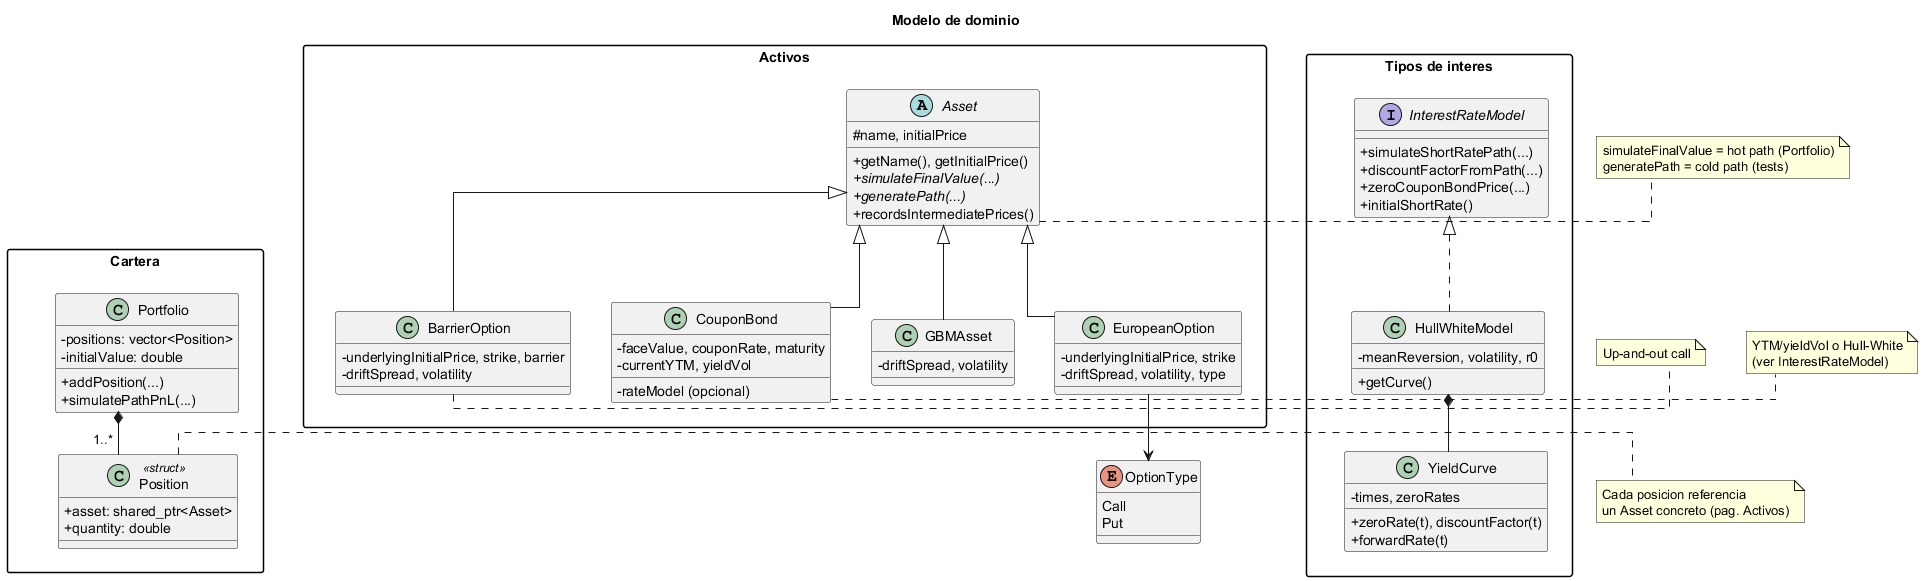
\includegraphics[width=\textwidth]{graphics/uml/uml_dominio.png}
  \caption{Modelo de dominio del motor: jerarquía de activos, agregación en cartera (\texttt{Portfolio}--\texttt{Position}) y modelado de tipos de interés.}
  \label{fig:uml-dominio}
\end{figure}

\begin{figure}[htbp]
  \centering
  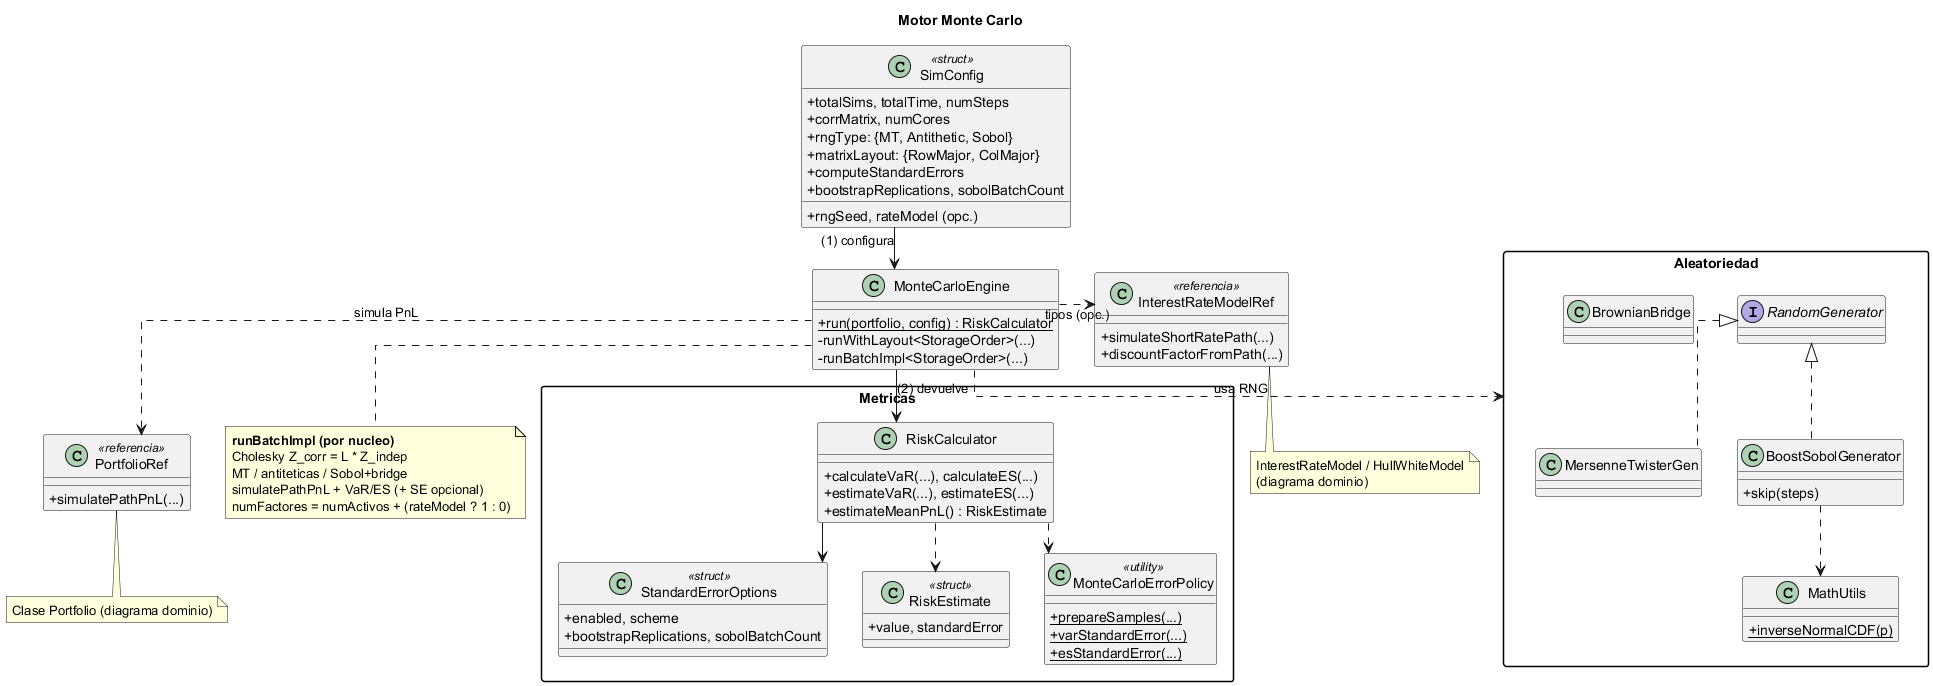
\includegraphics[width=\textwidth]{graphics/uml/uml_motor.png}
  \caption{Motor Monte Carlo: configuración (\texttt{SimConfig}), orquestación (\texttt{MonteCarloEngine}), generación aleatoria y cálculo de métricas de riesgo.}
  \label{fig:uml-motor}
\end{figure}

Este desacoplamiento arquitectónico garantiza flexibilidad funcional.
Modificar el horizonte temporal (p.\,ej.\ 1 día, 10 días o 1 año), el número de simulaciones, el generador aleatorio, la matriz de correlación o el modelo de tipos se reduce a reconfigurar \texttt{SimConfig} en los entornos de prueba (\texttt{test\_acciones.cpp} y \texttt{test\_montecarloEngine.cpp}), sin alterar la lógica interna del motor ni recompilar binarios de producción más allá de la reejecución de los tests de integración.

% Rutas de figuras relativas al directorio raíz del TFM (ajustar \graphicspath si procede).
% Alternativa vectorial: uml_dominio_sin_titulo.pdf, uml_motor.pdf (exportar con PlantUML).

\subsection{Arquitectura del sistema propuesto y flujo de ejecución}
\label{subsec:arquitectura-sistema}

Para evitar el acoplamiento rígido de componentes---un defecto habitual en motores de simulación académicos---, el sistema se ha diseñado bajo un enfoque modular y orientado a objetos, distribuyendo las responsabilidades en bibliotecas independientes (\texttt{Asset}, \texttt{Portfolio}, \texttt{Random}, \texttt{InterestRate}, \texttt{MontecarloEngine} y \texttt{Metrics}). El flujo de vida del dato dentro del motor puede estructurarse en tres fases secuenciales: \emph{configuración}, \emph{orquestación y simulación}, y \emph{análisis de riesgo sobre la distribución empírica de P\&L} (cuantiles y métricas de cola).

A continuación se detallan las responsabilidades de los módulos principales. La Figura~\ref{fig:uml-dominio} recoge el \emph{modelo de dominio}; la Figura~\ref{fig:uml-motor}, el \emph{motor de simulación} y las métricas asociadas.

\begin{itemize}
  \item \textbf{Cápsula de configuración (\texttt{SimConfig}).}
  Estructura de datos ligera que centraliza los parámetros de la simulación y elimina variables codificadas en el código (\emph{hardcoded}).
  Almacena el horizonte temporal (\texttt{totalTime}), el número de pasos (\texttt{numSteps}), el tamaño muestral (\texttt{totalSims}), la matriz de correlación (\texttt{corrMatrix}), el paralelismo (\texttt{numCores}), el generador aleatorio (\texttt{rngType}, \texttt{rngSeed}), el \emph{layout} de la matriz de shocks (\texttt{matrixLayout}) y, de forma opcional, un modelo de tipos de interés (\texttt{rateModel}) y la estimación de errores estándar de VaR/ES (\texttt{computeStandardErrors}, \texttt{bootstrapReplications}, \texttt{sobolBatchCount}).
  Todos estos campos residen en memoria; \texttt{SimConfig} no gestiona rutas de ficheros de mercado.

  \item \textbf{Modelización de activos (\texttt{Asset} y derivadas).}
  La clase base abstracta \texttt{Asset} define la interfaz polimórfica de cualquier factor de riesgo.
  Las implementaciones concretas incluyen \texttt{GBMAsset} (movimiento browniano geométrico), \texttt{EuropeanOption}, \texttt{BarrierOption} (up-and-out call) y \texttt{CouponBond} (modo YTM o precio vía modelo de tipos).
  El método \texttt{simulateFinalValue} constituye el \emph{hot path} invocado por la cartera;  \texttt{generatePath} se reserva para tests y análisis (\emph{cold path}).
  Esta jerarquía permite que el motor sea agnóstico respecto al modelo estocástico de cada instrumento.

  \item \textbf{Agregación en cartera (\texttt{Portfolio}, \texttt{Position}).}
  \texttt{Portfolio} agrupa posiciones (\texttt{Position}), cada una con un \texttt{shared\_ptr<Asset>} y una cantidad.
  El método \texttt{simulatePathPnL} calcula el P\&L de una trayectoria: valora cada activo mediante \texttt{simulateFinalValue}, aplica descuento opcional con \texttt{InterestRateModel} y resta el valor inicial de la cartera.

  \item \textbf{Tipos de interés (\texttt{InterestRateModel}, \texttt{HullWhiteModel}).}
  Interfaz abstracta para simular la trayectoria del tipo corto, descontar flujos y valorar bonos.
  La implementación \texttt{HullWhiteModel} compone una \texttt{YieldCurve} de mercado.
  Su uso es opcional: cuando \texttt{SimConfig.rateModel} está activo, la matriz de correlación incorpora un factor adicional para el driver browniano del tipo.

  \item \textbf{Aleatoriedad (\texttt{RandomGenerator} y utilidades).}
  \texttt{MersenneTwisterGen} y \texttt{BoostSobolGenerator} implementan la interfaz \texttt{RandomGenerator}.
  El motor selecciona el generador según \texttt{rngType}: Mersenne Twister, variables antitéticas (pares $(Z,-Z)$) o secuencias de Sobol.
  En el modo Sobol, \texttt{BoostSobolGenerator} transforma uniformes cuasi-aleatorios mediante \texttt{MathUtils::inverseNormalCDF} y \texttt{MonteCarloEngine} aplica \texttt{BrownianBridge} por factor antes de la correlación.

  \item \textbf{Núcleo de orquestación (\texttt{MonteCarloEngine}).}
  Punto de entrada \texttt{run(const Portfolio\&, const SimConfig\&)}.
  Recibe una cartera ya construida (no la instancia), descompone la correlación con Cholesky ($Z_{\mathrm{corr}} = L Z_{\mathrm{indep}}$), paraleliza batches con \texttt{std::async} y coordina RNG, trayectorias de tipos y llamadas a \texttt{Portfolio::simulatePathPnL}.
  Es aquí donde se integran las técnicas de reducción de varianza y el bucle crítico de Monte Carlo.

  \item \textbf{Consumidor de riesgo (\texttt{RiskCalculator}, \texttt{MonteCarloErrorPolicy}).}
  Módulo de análisis \emph{posterior} a la simulación.
  Recibe el \emph{vector} de P\&L simulados (no una matriz), los ordena y calcula VaR$_\alpha$ y ES$_\alpha$ empíricos para $\alpha \in (0,1)$.
  Cuando \texttt{computeStandardErrors} está activo, \texttt{MonteCarloErrorPolicy} estima errores estándar según el esquema asociado al \texttt{rngType} (muestras independientes, pares antitéticos o medias por lotes Sobol), devolviendo \texttt{RiskEstimate} con valor y error.
  Las operaciones estadísticas quedan así aisladas de la lógica de simulación.
\end{itemize}

Como se aprecia en las Figuras~\ref{fig:uml-dominio} y~\ref{fig:uml-motor}, la interacción entre componentes modela el flujo de dependencias del software: el dominio financiero (activos, cartera y tipos) se desacopla del motor, que a su vez delega las métricas en \texttt{Metrics}.
El orquestador central gobierna el ciclo de vida de la simulación sin violar el principio de responsabilidad única.

\begin{figure}[htbp]
  \centering
  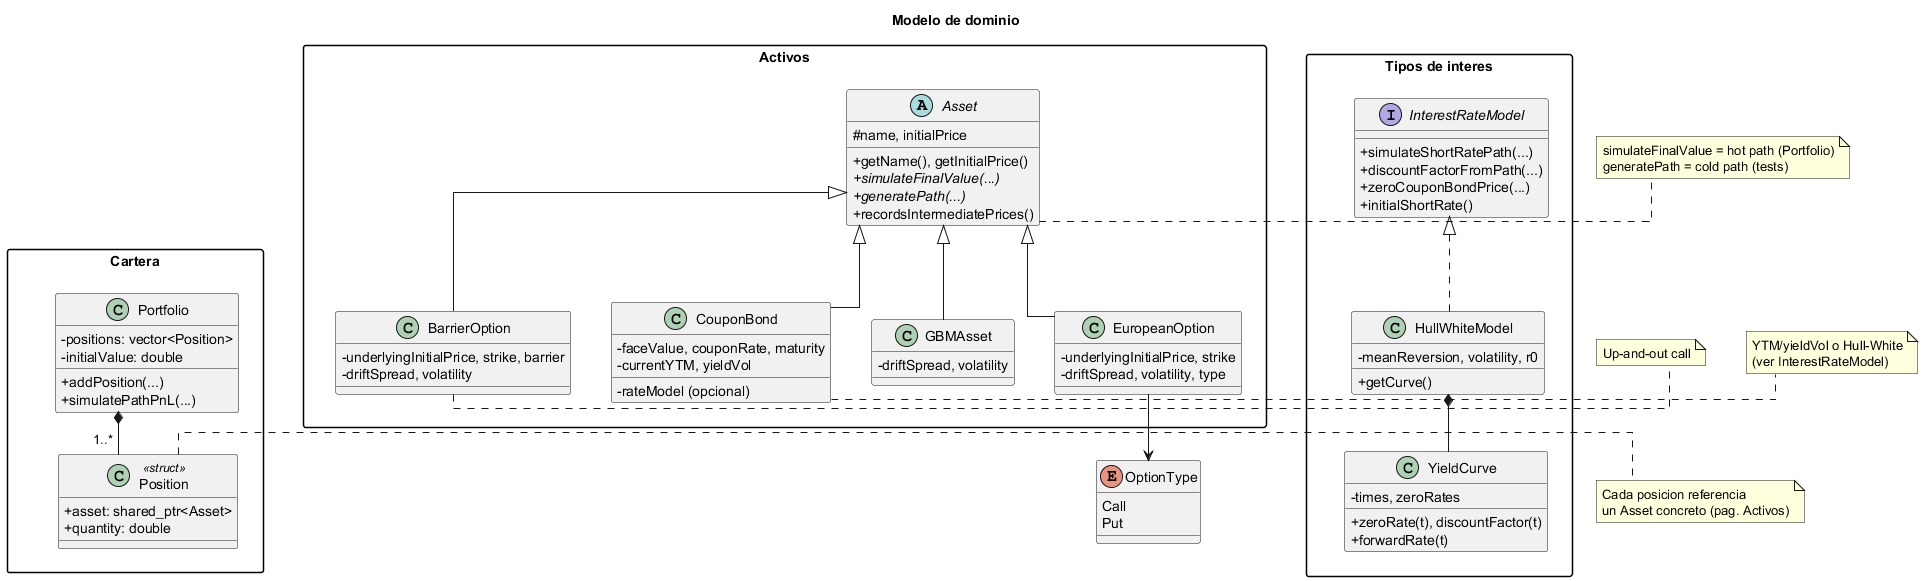
\includegraphics[width=\textwidth]{graphics/uml/uml_dominio.png}
  \caption{Modelo de dominio del motor: jerarquía de activos, agregación en cartera (\texttt{Portfolio}--\texttt{Position}) y modelado de tipos de interés.}
  \label{fig:uml-dominio}
\end{figure}

\begin{figure}[htbp]
  \centering
  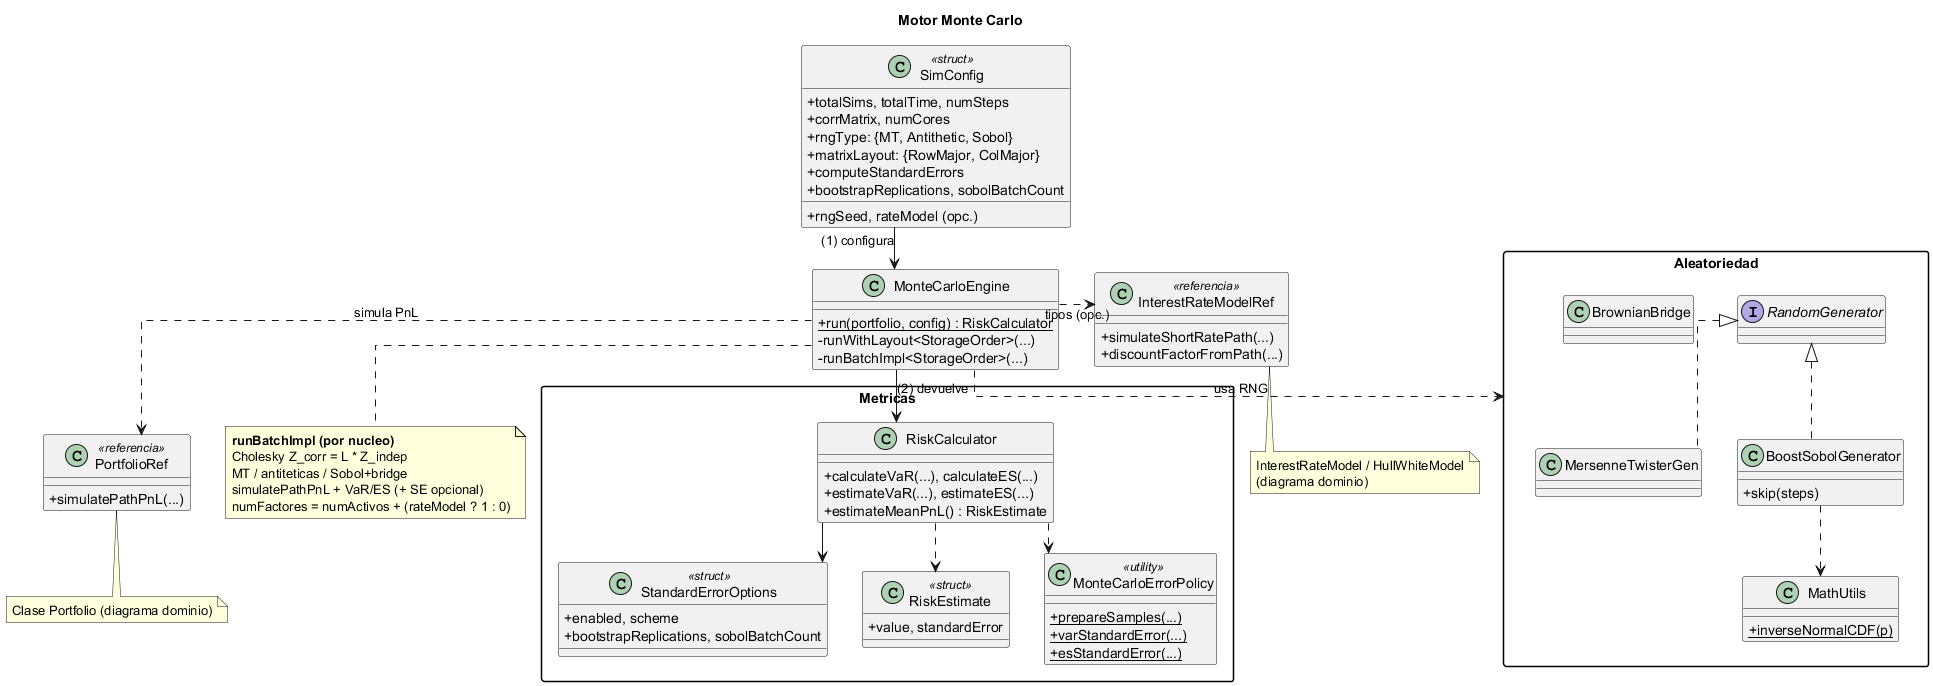
\includegraphics[width=\textwidth]{graphics/uml/uml_motor.png}
  \caption{Motor Monte Carlo: configuración (\texttt{SimConfig}), orquestación (\texttt{MonteCarloEngine}), generación aleatoria y cálculo de métricas de riesgo.}
  \label{fig:uml-motor}
\end{figure}

Este desacoplamiento arquitectónico garantiza flexibilidad funcional.
Modificar el horizonte temporal (p.\,ej.\ 1 día, 10 días o 1 año), el número de simulaciones, el generador aleatorio, la matriz de correlación o el modelo de tipos se reduce a reconfigurar \texttt{SimConfig} en los entornos de prueba (\texttt{test\_acciones.cpp} y \texttt{test\_montecarloEngine.cpp}), sin alterar la lógica interna del motor ni recompilar binarios de producción más allá de la reejecución de los tests de integración.
